\begin{figure*}[!ht]
\centering
\subfigure[CDF of Backers Distribution] % caption for subfigure b
{
    \label{fig:CDF-backers}
    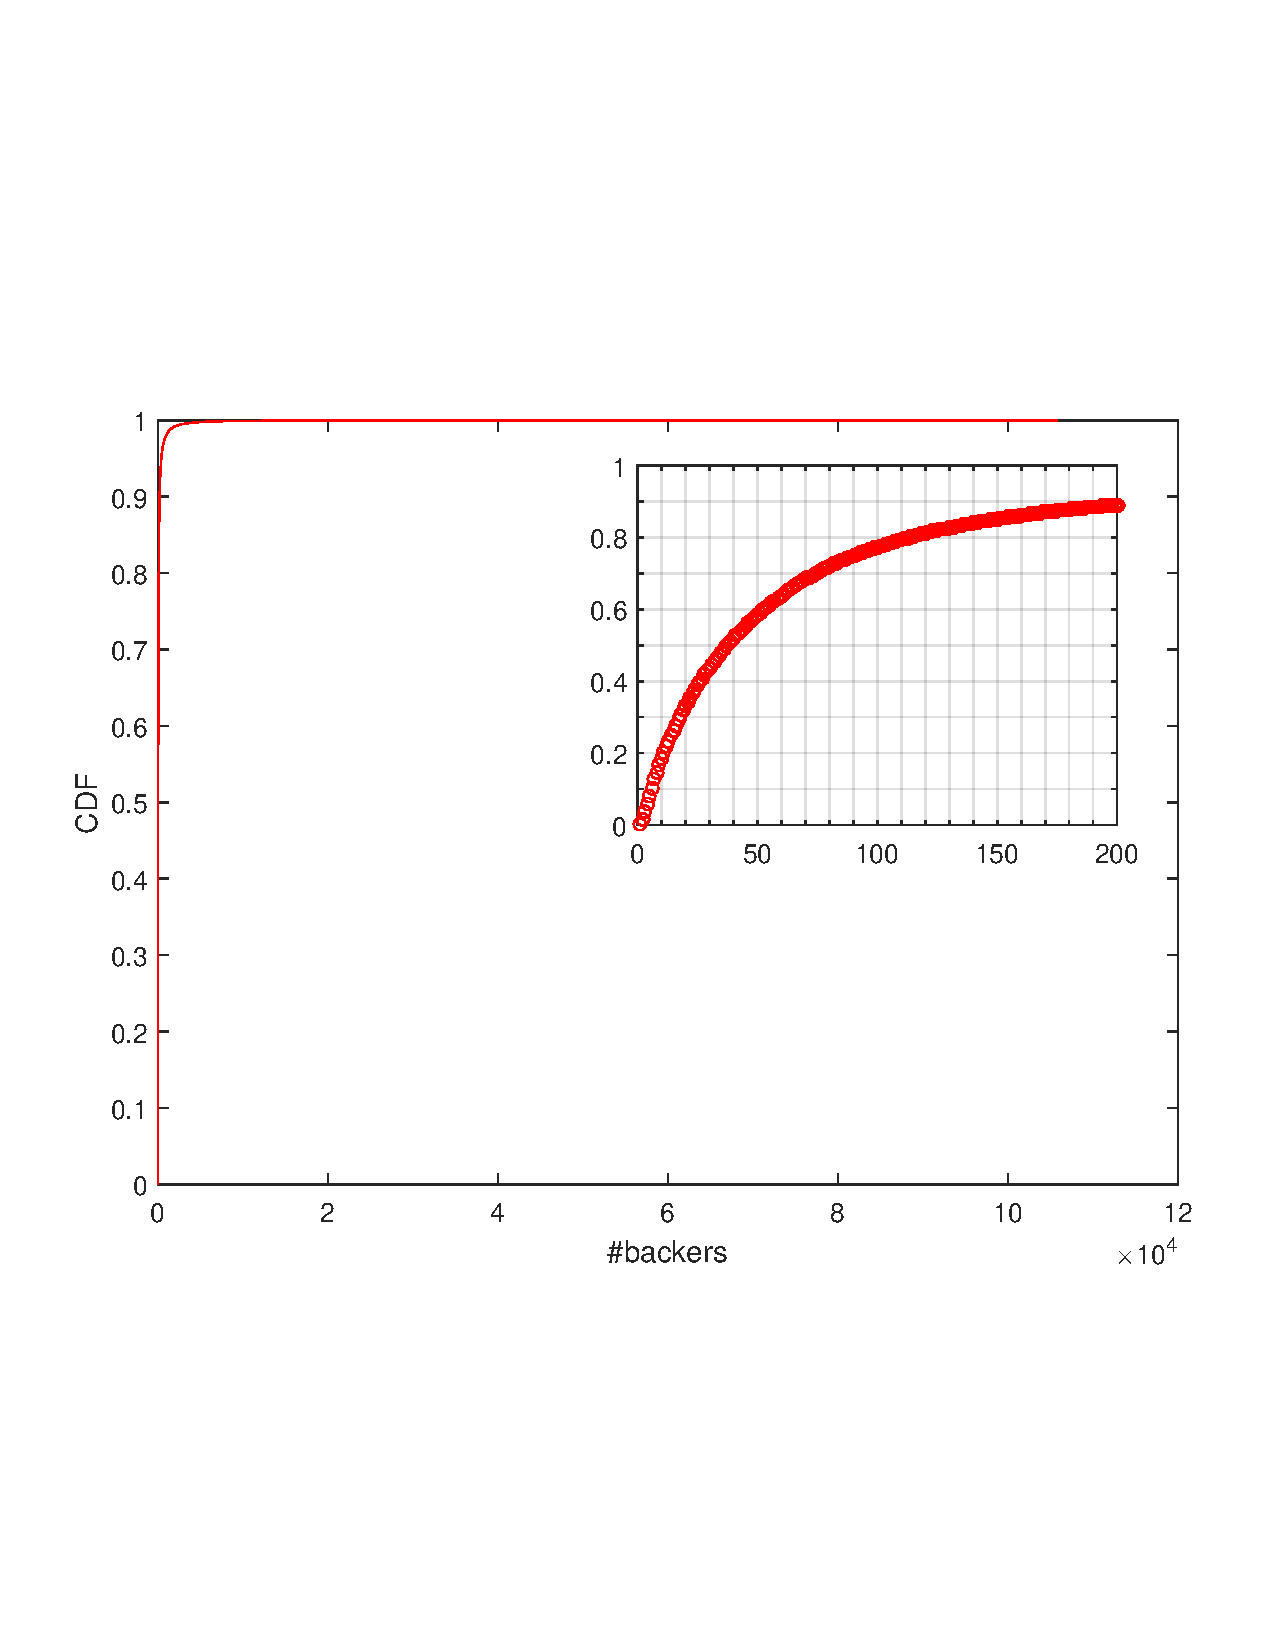
\includegraphics[width=0.47\linewidth]{figs/CDF-backers.pdf}
}
%\hspace{0.03cm}
\subfigure[CDF of Funding Distribution] % caption for subfigure a
{
    \label{fig:CDF-funding}
    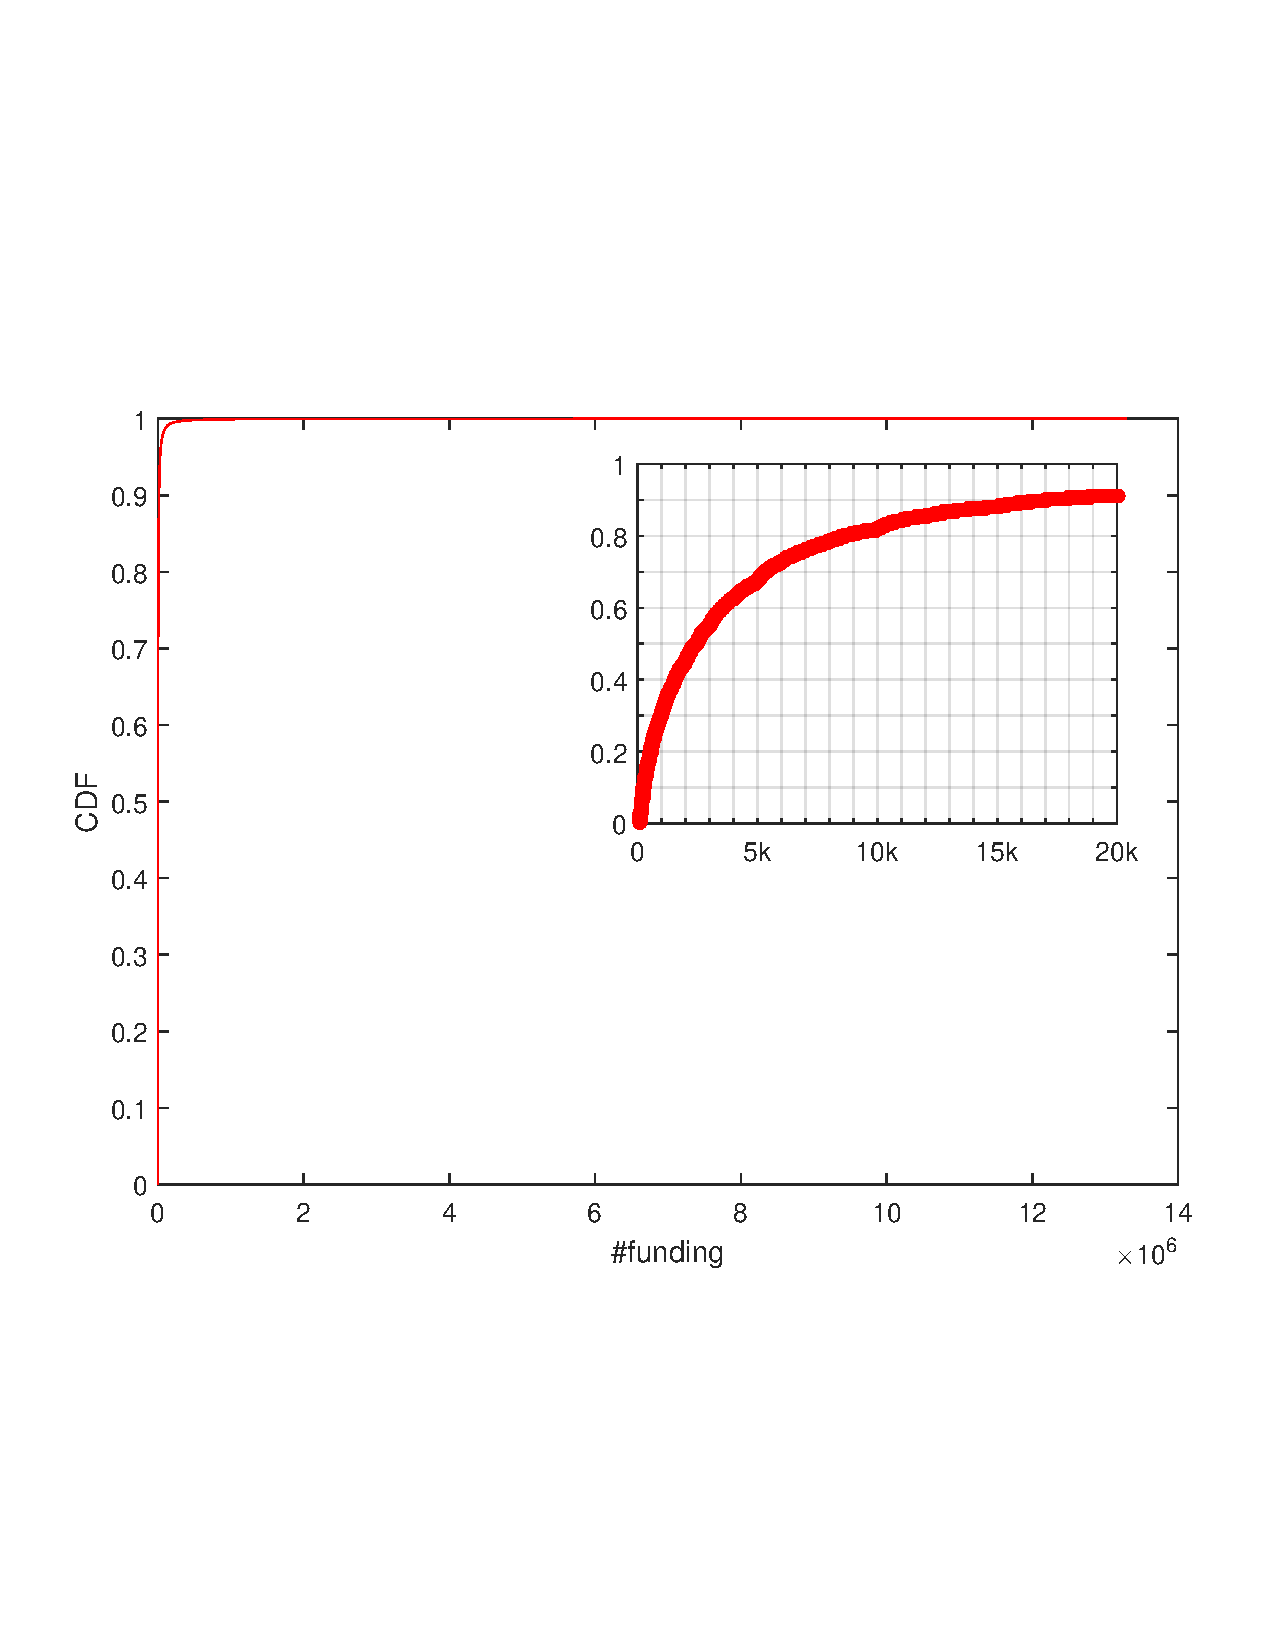
\includegraphics[width=0.47\linewidth]{figs/CDF-funding.pdf}
}
\caption{Cumulative Distribution Function of Backers and Funding}
\label{fig:CDF-overall} % caption for the whole figure
%\vspace{-10pt}
\end{figure*}

\section{Analysis}


In statistics, linear regression is an approach for modeling the relationship between a dependent variable y and one or more explanatory variables denoted X. In this paper, there are more than one explanatory variable, the process is called multiple linear regression.

In linear regression, the relationships are modeled using linear predictor functions whose unknown model parameters are estimated from the data. Such models are called linear models.

As Figure \ref{fig:CDF-overall} shown, only 10\% of total project obtains more than 200 backers and \$20,000 funding. In other words, majority of project could not achieve such a large number of backers and funding. It confirms that it is essential to success to know how many backers will fund and how much money will be collected.

\begin{figure*}[!ht]
\centering
  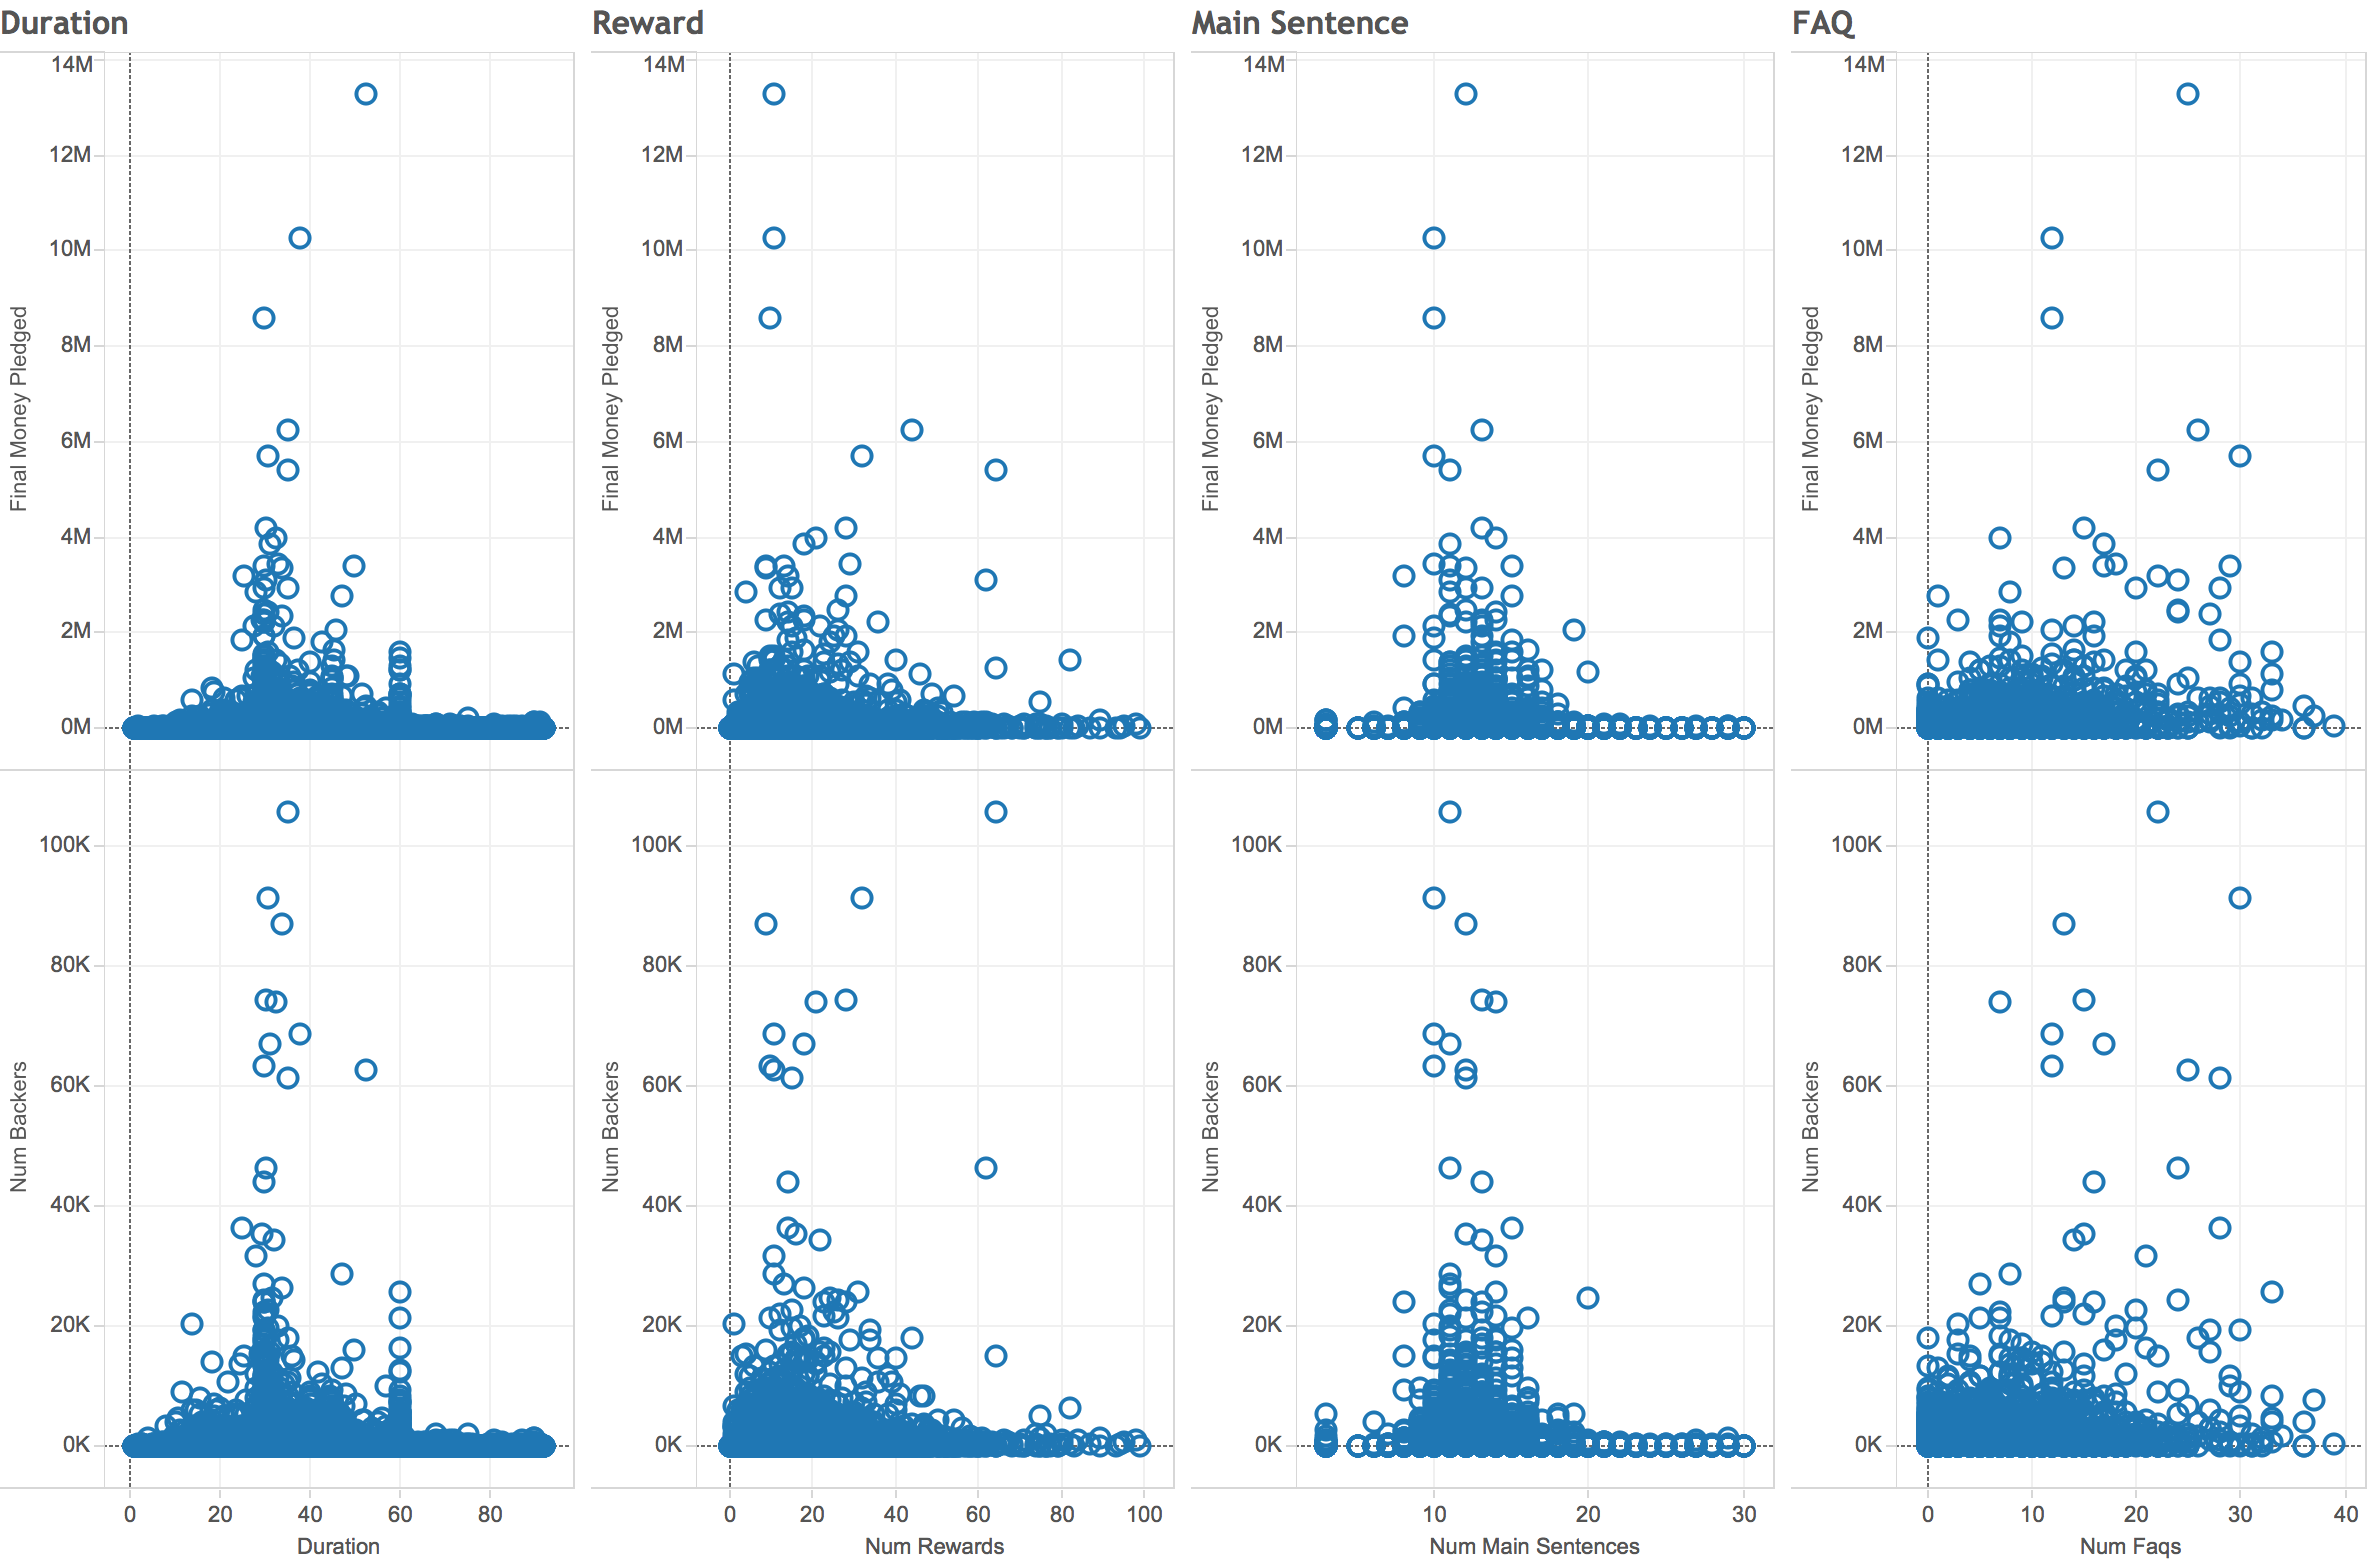
\includegraphics[width=1\textwidth]{figs/scatter_money_backer}
    \caption{Scatter plot between available features and Final pledged money, backer}
  \label{fig:scatterMoneyBacker}
\end{figure*}

Before discovering a model, we would like to see relation between major features and the number of backers, finally pledged money. In Figure \ref{fig:scatterMoneyBacker}, it gives that there is not specific linear relation between independent variables such as project duration, description length, the number of rewards, and the number of frequently asked question.

It is likely to have a shape of normal distribution in that there are more backers and participation in fund with middle of independent variables. In case of duration, there are many marks near point of ``30''. It has similar pattern in relation on the number of reward. This phenomenon makes hard to make model because the different dependent variables from the same independent variable. It requires to find some transformation method to fit a model.

\begin{figure}[!ht]
\centering
  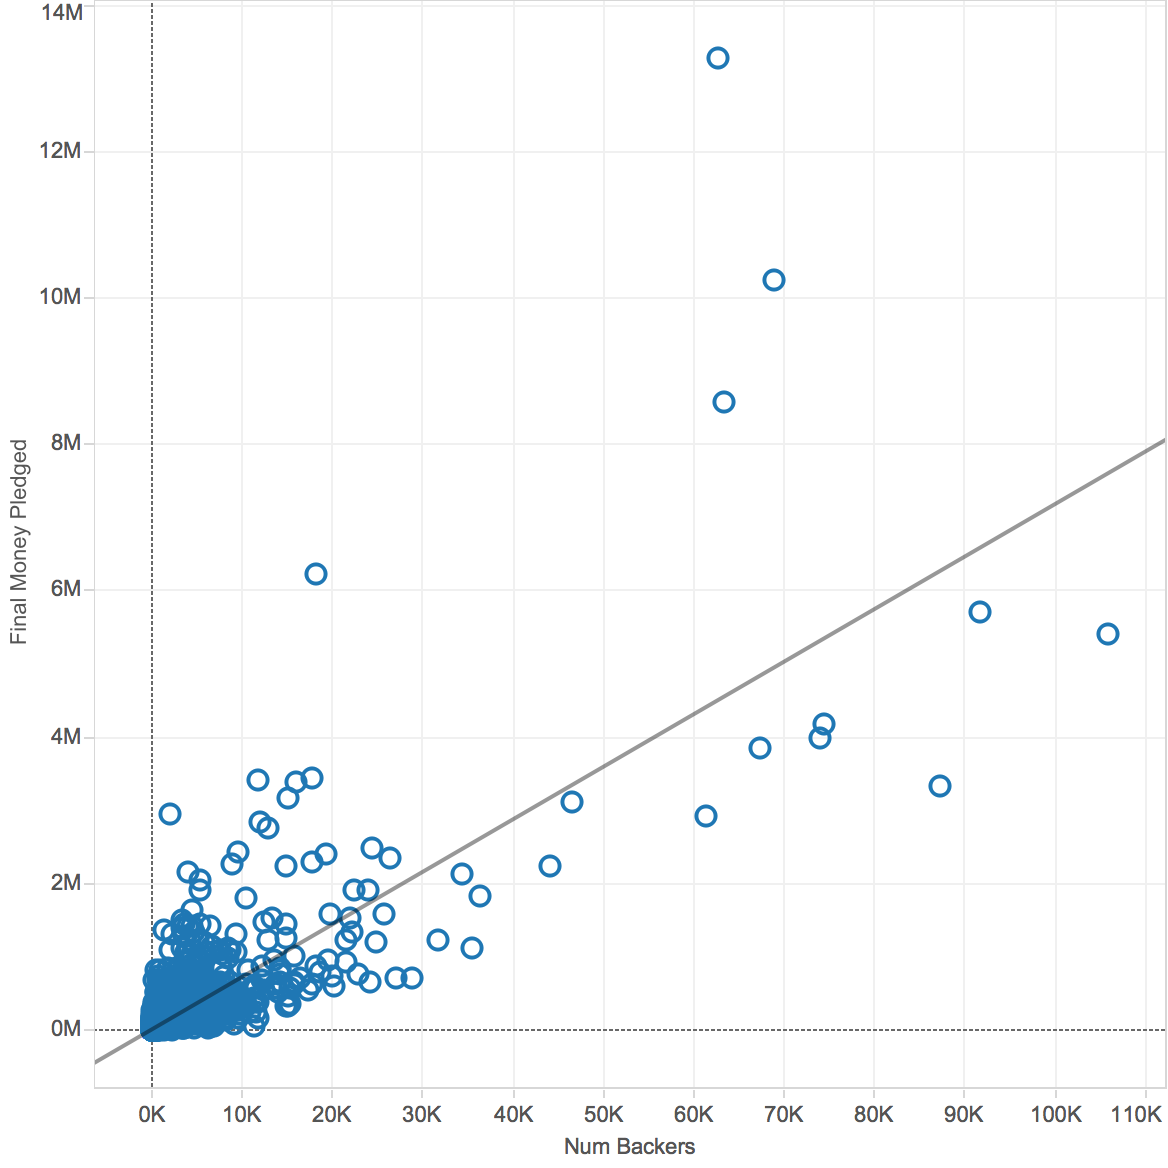
\includegraphics[width=0.48\textwidth]{figs/backers_money}
    \caption{Scatter plot between Final pledged money and backer}
  \label{fig:scatterMoneyBacker}
\end{figure}

There are similar patterns of distribution whether response variable is final pledged money or the number of backers. To understand this phenomenon, it is need to investigate relationship between them. It is obvious that there should be positive relation between the number of backers and pledged money. When more users are involved in a specific project, it is natural that the project have more fund in the last.

Figure \ref{fig:scatterMoneyBacker} shows relation between the number of backers and final pledged money. 
Linear regression line is represented with the below equation.

\begin{equation}
Final Money Pledged = 71.8998*Num Backers + 845.879	
\end{equation}
 
With significance level 0.05, the model is acceptable because its p-value is less than 0.0001. Besides, $R^2$ which provides a measure of how well future outcomes are likely to be predicted by the regression model and how well the regression line fits real data.is 0.6321. It represents that this model with the number of backers explains 63.21\% variance of final pledged money.

\begin{figure}[!ht]
\centering
  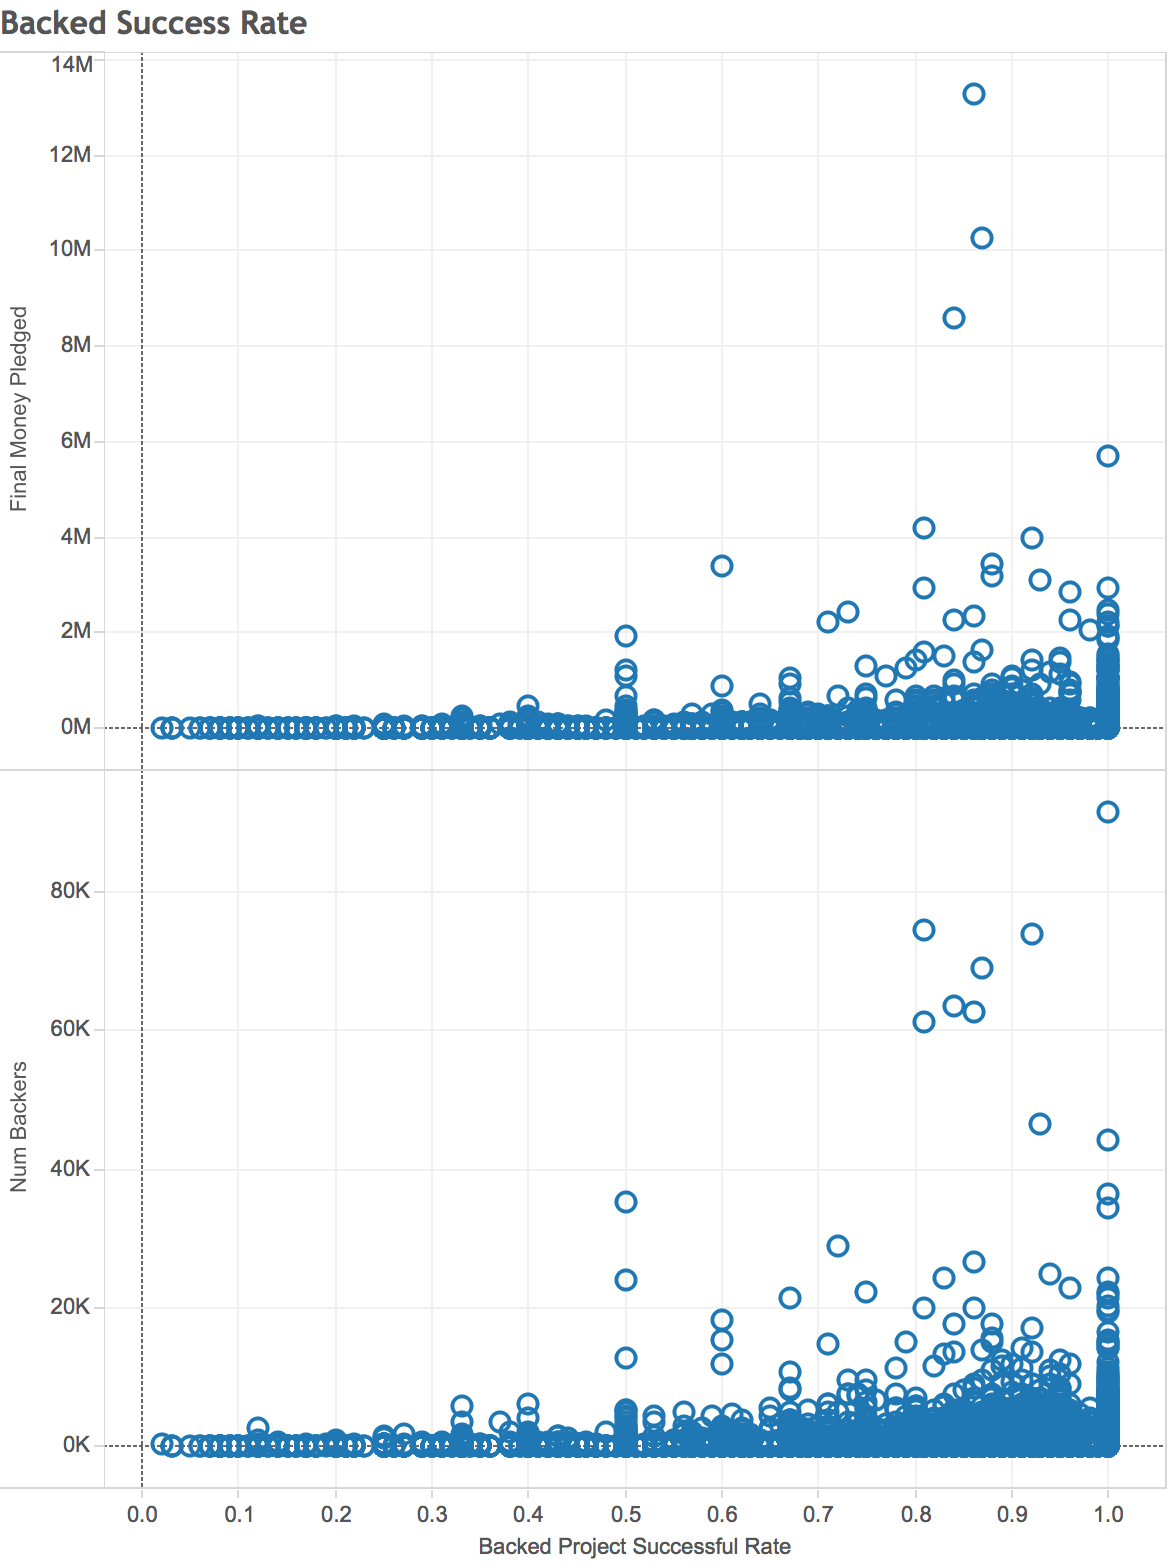
\includegraphics[width=0.48\textwidth]{figs/successfulrate}
    \caption{Scatter plot between Final pledged money and backer with previous success project rate}
  \label{fig:scatterSuccessRate}
\end{figure}

Figure \ref{fig:scatterSuccessRate} shows relation between final pledged money and the number of backer with previous project success rate. It represents that the more success rate in previous project, the more chance to attract backers which leads to get more financial support.This could not fully guarantee successful modeling but it point out one of features which affect project success.

